
% example exists at http://www.texample.net/tikz/examples/marketing-distribution-channel/
\begin{figure}
\centering
\begin{tikzpicture}[node distance=1cm, auto]  
\tikzset{
    mynode/.style={rectangle,rounded corners,draw=black, top color=white, bottom color=yellow!50,very thick, inner sep=1em, minimum size=3em, text centered},
    myarrow/.style={->, >=latex', shorten >=1pt, thick},
    mylabel/.style={text width=7em, text centered} 
}  
\node[mynode] (backend) {Backend};  
\node[below=3cm of backend] (dummy) {}; 
\node[mynode, left=of dummy] (mobile) {Mobile application};  
\node[mynode, right=of dummy] (web) {Web application};

\draw[myarrow] (backend.south)  -- ++(0,-1) -|  (mobile.north);
\draw[myarrow] (mobile.north)  -- ++(0,1.506) -|  (backend.south);
\draw[myarrow] (backend.south)  -- ++(0,-1) -|  (web.north);
\draw[myarrow] (web.north)  -- ++(0,1.506) -|  (backend.south);
% There is a slight overlap of the arrows with the (manufacturer) south edge
% because creating the offset in another way didn't compile. 

\end{tikzpicture} 
\medskip
\caption{Seperate mobile and web application connected with a common backend.} 
\end{figure}

\begin{figure}
\centering
\begin{tikzpicture}[node distance=1cm, auto]  
\tikzset{
    mynode/.style={rectangle,rounded corners,draw=black, top color=white, bottom color=yellow!50,very thick, inner sep=1em, minimum size=3em, text centered},
    myarrow/.style={->, >=latex', shorten >=1pt, thick},
    mylabel/.style={text width=7em, text centered} 
}  
\node[mynode] (backend) {Backend};  
\node[below=3cm of backend] (dummy) {}; 
\node[mynode, left=of dummy] (mobile) {Mobile application};  
\node[mynode, right=of dummy] (web) {Web application};

\draw[myarrow] (backend.south)  -- ++(0,-1) -|  (web.north);
\draw[myarrow] (web.north)  -- ++(0,1.506) -|  (backend.south);
\draw[myarrow] (web.west)  -- (mobile.east);
\draw[myarrow] (mobile.east)  -- (web.west);
% There is a slight overlap of the arrows with the (manufacturer) south edge
% because creating the offset in another way didn't compile. 

\end{tikzpicture} 
\medskip
\caption{Seperate mobile and web application connected with a common backend.} 
\end{figure}

% example exists at http://www.texample.net/tikz/examples/tree/
\begin{figure}
\centering
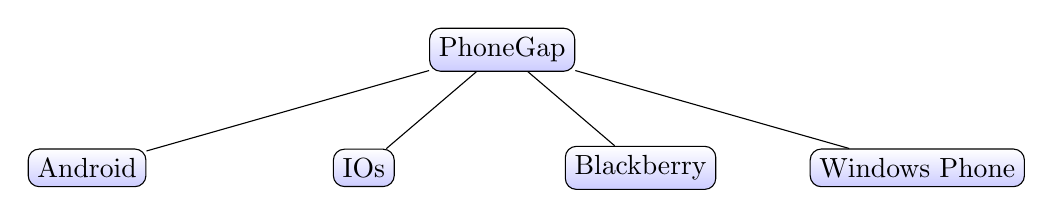
\begin{tikzpicture}[sibling distance=10em,
  every node/.style = {shape=rectangle, rounded corners,
    draw, align=center,
    top color=white, bottom color=blue!20}]]
  \node {PhoneGap}
    child { node {Android} }
    child { node {IOs} }
    child { node {Blackberry} }
    child { node {Windows Phone} };
\end{tikzpicture}
\medskip
\caption{PhoneGap can be compiled into multiple plattoforms.} 
\end{figure}